\documentclass{article}

\usepackage{graphicx} % Required for inserting images
\usepackage{verbatim}
\usepackage[utf8]{inputenc}
\usepackage{graphicx}
\usepackage{float}
\usepackage{fancyvrb}
\usepackage{varwidth}
\usepackage{amsmath}
\usepackage{siunitx}



\title{EE736-Stochastic Optimization Project\\ Reinforcement Learning in Finance}
\author{Mohit\\20D070052 }
\date{April 2023}

\begin{document}

\maketitle
\begin{figure}[H]
\begin{center}

\includegraphics[scale = 0.2]{LOGO.jpeg}
\end{center}
\end{figure}
\section{Student Details}
\begin{tabular}{ l l  }
 Name: & Mohit \\ 
 Roll No: & 20D070052  \\  
\end{tabular}
\newpage

\section{Papers Reviewed}
\begin{itemize}
\item Recent Advances in Reinforcement Learning in Finance
\item Reinforcement Learning in Economics and Finance
\item Modern Perspectives on Reinforcement Learning in Finance
\end{itemize}

\section{Modern Perspectives on Reinforcement Learning in Finance}
\subsection{Introduction}
This article discusses the use of reinforcement learning (RL) techniques for solving intertemporal choice problems in finance. Intertemporal choice problems involve decision making where the costs and benefits are spread over time and the choices made at one time affect the possibilities available at other times. The article explains that dynamic programming (DP) is commonly used to solve these problems, but it relies on several assumptions that may not be true in practice. RL provides a way to overcome these issues by building agents that can act intelligently and efficiently solve problems. The article discusses the use of value functions, which are mathematical expectations in a certain probability space, as a useful mathematical object for RL. It also highlights that RL has developed independently from classical utility theory in economics and finance and provides a way to train artificial agents to optimize cumulative reward over time through "trial and error" by receiving feedback on the reward resulting from each action taken. many stochastic systems in finance are complex and it is difficult to derive or estimate correct expressions of their dynamics. This is referred to as the curse of modeling. The article concludes by mentioning successful applications of RL in recent years, such as creating superhuman video game players and the world's best Go player.

\subsection{Markov Decision Processes}
An interesting figure is included here:
\begin{figure}[H]
\begin{center}
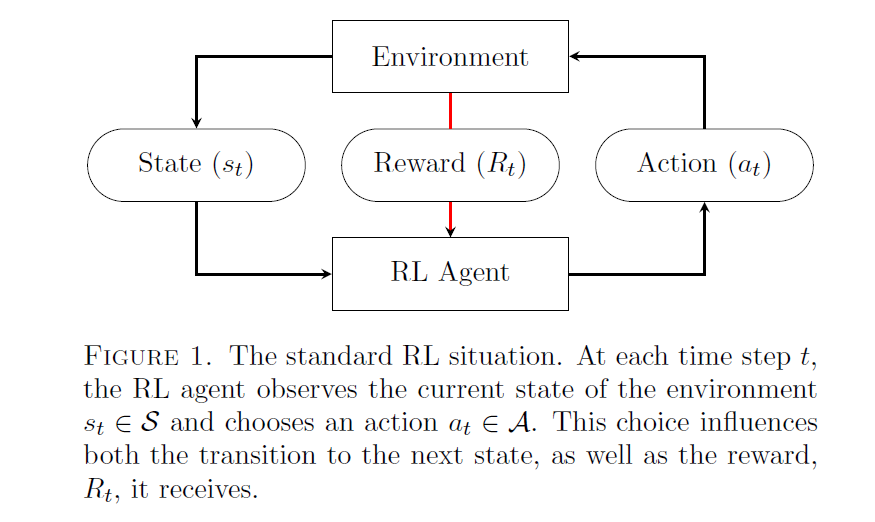
\includegraphics[scale = 0.5]{MDP.png}
\end{center}
\end{figure}

\subsection{Value Functions and Policies}
The action-value function is the expected goal function, assuming we start in state s, take action a and then follow some fixed policy $\pi$ from then on\\
\begin{center}
$q_\pi (s,a) = E[G_t]$ starting from s, taking a, then following $\pi $
\end{center}


\begin{figure}[H]
\begin{center}
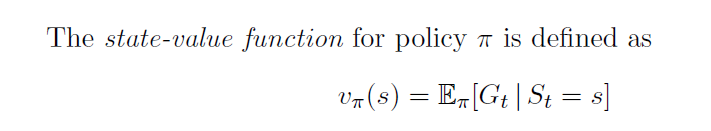
\includegraphics[scale = 0.5]{State.png}
\end{center}
\end{figure}

An optimal policy is defined to be one which is at least as good as any other policy. There need not be a unique optimal policy, but all optimal policies share the same optimal state-value function.

\subsection{The Bellman Equations }

It is straightforward to establish that the optimal state-value function and action-value function satisfy the Bellman equations.

\begin{figure}[H]
\begin{center}
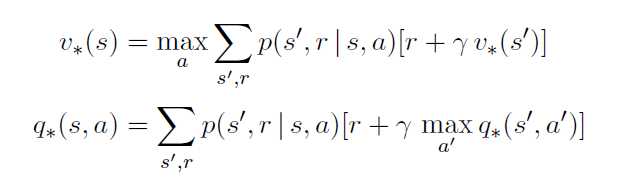
\includegraphics[scale = 0.5]{Bell.png}
\end{center}
\end{figure}

where the sum over s, r denotes a sum over all states s and all rewards r.\\
RL methods which focus on learning the association Y = f(X) + noise with (X, Y ) as above are referred to as function approximation by Sutton and Barto (2018).

\subsection{Some Decision Problems in Trading}
\subsubsection{Replication of a derivative contract}
Given a derivative contract, suppose there is a dynamic trading strategy which gives the same payout as this contract in every state of the world; such world-states are usually referred to as Arrow-Debreu states in economics. In other words,
this strategy is a replicating strategy. Suppose the policy $\pi$ is to follow the replicating strategy. Then the no arbitrage price of the option is\\
\begin{center}
$v_\pi (s_0)$
\end{center}
where $s_0$ is the state of the world today. Note that this applies to any state-contingent claim, and is not limited to Black-Scholes-Merton (BSM) or lognormal models.

\subsubsection{Optimal order execution}
Let us consider liquidating an order of size X using the framework of Almgren and Chriss (1999) and Almgren and Chriss (2001). Almgren and Chriss suggest to determine the sequence of child orders by maximizing expected mean-variance utility. In this case, the value function is the expected integrated revenue and variance

\begin{figure}[H]
\begin{center}
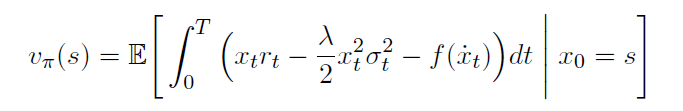
\includegraphics[scale = 0.5]{Ex2.png}
\end{center}
\end{figure}

\subsubsection{Dynamic portfolio rebalancing with time-dependent return predictions and market impact costs}
Buy-side quant traders are interested in maximizing their expected utility of wealth subject to trading costs. Using
mean-variance utility results in the model by Gˆarleanu and Pedersen (2013). This approach is conceptually similar to that of optimal order liquidation above, but with the added complexity of time-varying return predictions (“alpha”).

\subsubsection{Portfolio allocation subject to capital gains taxes}
Previous Example can be extended to include capital gains and other taxes, resulting in a dynamic portfolio rebalancing model for after-tax investing (see, for example, Constantinides (1984), Garlappi, Naik, and Slive (2001), Dammon, Spatt, and Zhang (2004), DeMiguel and Uppal (2005), and Haugh, Iyengar, and Wang (2016)). Just as in the previous example, RL methods can in principle be applied to solve these after-tax problems.

\subsection{Economically Motivated Reward Signals}
RL possesses a rather obvious connection with games and game theory and hence with game-theoretic approaches to economics. The player is the “agent” and the “environment” consists of the other players or the simulated environment of the game. For many games including backgammon, Go and some video games, the best player in the world is an AI trained using reinforcement learning (see, for example, Mnih et al. (2013), Mnih et al. (2015), Tian and Zhu (2015), and Silver et al. (2017)). Von Neumann and Morgenstern (1945) show that if a decision-maker\\
(i) is faced with risky (probabilistic) outcomes of different choices and\\
(ii) has preferences satisfying four axioms of “rational behavior”\\

In finance, an optimal trading strategy is usually defined as a strategy that maximizes expected utility of future wealth, where future wealth is the sum of a number of wealth increments over shorter time periods. Hence, to find the optimal trading strategy we seek to solve the problem

\begin{figure}[H]
\begin{center}
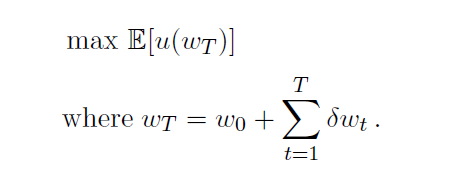
\includegraphics[scale = 0.5]{Mod.png}
\end{center}
\end{figure}


Ergodicity means intuitively that where the MDP starts, or any early decision made by the RL agent, can have only a
temporary effect.

\subsection{States and Actions for Trading Problems}
The state variable st is a data structure which intuitively must contain everything the RL agent needs to make a trading decision and nothing else. Candidate state variables include:\\
(i) the current position or holding in the security,\\
(ii) the values of any signals which are believed to be predictive,\\
(iii) the current state of the market, including current price and any relevant microstructure / limit-order book details, and\\
(iv) if contingent claims are involved, additional variables such as time to expiry to properly define the contract.\\

In trading problems, the most obvious choice for the action at is the number of securities to trade. If the RL agent’s interaction with the market microstructure is important, then there will typically be more choices to make and hence a larger action space. For example, the RL agent could decide which execution algorithm to use, whether to cross the spread or be passive, its target participation rate, etc. If one of the securities is a contingent claim, there may be additional actions available, such as early exercise or, more generally, a pre-specified set of dates or other conditions at which the user can exercise various kinds of optionality.

\subsection{Trading Mean-Reversion with RL}
We extend Ritter (2017) by introducing a continuous state space formulation and providing an explicit graphical representation of the resulting value function. We will see later from the value function that the RL agent has learned the existence of a notrade zone in a neighborhood around the equilibrium price.

The RL agent also does not know the trading cost. We charge a spread cost of one tick size for any trade. If the bid-offer spread were equal to two ticks, then this fixed cost would correspond to the slippage incurred by an aggressive fill which crosses the spread to execute. If the spread is only one tick, then our choice is overly conservative. In this article we will use the following representation of the spread cost\\
\begin{center}
SpreadCost($\delta$n) = TickSize · |$\delta$n|\\
ImpactCost($\delta$n) = ($\delta$n)2 × TickSize/LotSize .\\
Taken together, the total trading cost becomes\\
Cost($\delta$n) = multiplier × (SpreadCost($\delta$n) + ImpactCost($\delta$n) .\\
\end{center}

We use an ensemble of model trees as our nonlinear regression learner, but that is certainly not the only possible choice it is likely that an artificial neural network would work as well.

\begin{figure}[H]
\begin{center}
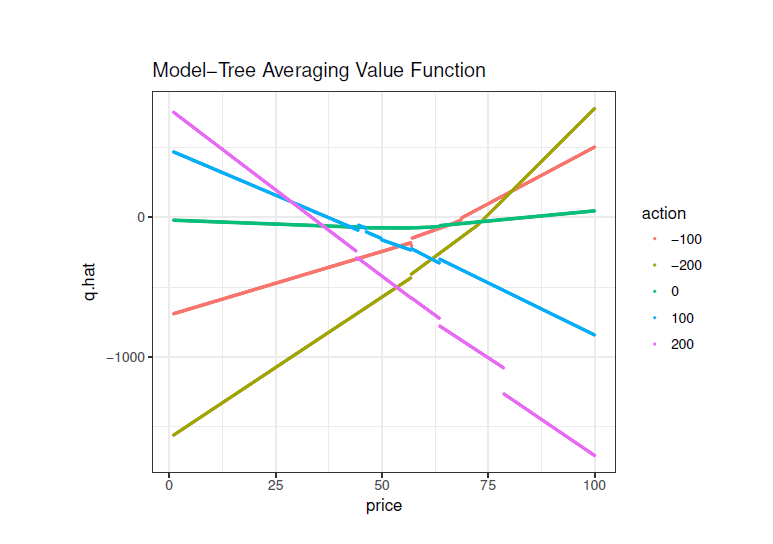
\includegraphics[scale = 0.5]{Avg.png}
\end{center}
\end{figure}

\begin{figure}[H]
\begin{center}
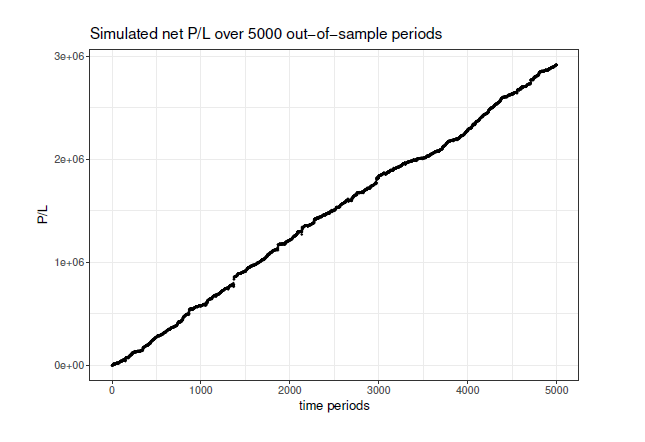
\includegraphics[scale = 0.5]{Sam.png}
\end{center}
\end{figure}

\subsection{Conclusion}
The article discusses the potential of reinforcement learning (RL) in solving modern financial problems, such as pricing and hedging of contingent claims, investment and portfolio allocation, market making, and optimization of tax consequences. RL allows for solving dynamic optimization problems in a "model-free" way, relaxing the assumptions needed for dynamic programming approaches. However, RL also poses challenges, such as correct model specification, acquisition of sufficient data, and generalization of RL models. The authors expect exciting new results connecting the fields of finance, machine learning, and numerical solutions of PDEs using RL as the common thread.

\section{Reinforcement Learning in Economics and Finance}
\subsection{Introduction}
Reinforcement learning is a type of learning where agents, animals, or robots adapt their behavior through experience to maximize rewards. It differs from other types of learning as it follows from feedback and experience rather than fixed training samples. Reinforcement learning has been used in behavioral psychology, ethology, and biology. It involves understanding how agents can learn to make optimal decisions through repeated experience while maximizing long-term rewards. Markov decision processes are used to solve the credit assignment problem by matching actions, states of the world, and rewards. The goal is to learn from past data to find an optimal policy. Reinforcement learning has many applications, including playing games such as chess or Go. Sequential machine learning techniques are used to compute the optimal policy.\\
The article discusses the relevance of reinforcement learning in sequential decision making and control, and its applications in various fields such as decision theory, game theory, and auction design. It describes the concept of learning from active experimentation and inferring the impact of interventions, and how this is useful in solving computationally difficult problems in economics. The article also presents recent advances in the field and their potential in modeling complex economic problems.\\

\subsection{From Machine to Reinforcement Learning}
Machine learning is a field that uses statistical methods to make decisions based on known properties learned from training data. The goal is to find a generalized predictive pattern that can be applied to new, unseen data. Reinforcement learning is a subset of machine learning that focuses on optimizing a criterion, such as maximizing a reward or minimizing a loss, by taking actions in an environment and receiving feedback in the form of rewards or penalties. In this approach, the emphasis is on minimizing regret, which is the difference between the expected reward and the actual reward received. This approach is useful in many real-world problems where the label associated with the problem is not always easy to identify.\\
In supervised learning, we prefer the name of excess risk, or excess loss. This notion of regret is particularly relevant in sequential learning, where your action at t depends on previous ones on t-1; t-2; ::: . In online (or sequential) learning, the regret is measured by the cumulative loss it suffers along its run on a sequence of examples.
Bandits and Reinforcement Learning deal with maximizing a reward, instead of minimizing a loss. Thus, we can re-write regret as the difference between the reward that could have been achieved and what was actually achieved according to a sequence of actions. Thus, minimizing a loss or maximizing a reward is the same optimization problem as minimizing the regret, as defined in Robbins

\subsection{Online Learning}
There exist several rules for aggregation, the most popular one is probably the Bernstein Online Aggregator (BOA Wintenberger 2017), which is optimal with bounded iid setting for the mean squared loss.
\begin{figure}[H]
\begin{center}
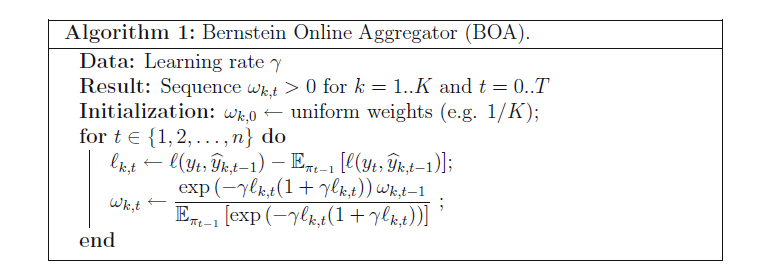
\includegraphics[scale = 0.5]{Algo.png}
\end{center}
\end{figure}

This technique, also called ensemble prediction, based on aggregation of predictive models, gives an easy way to improve forecasting by using expert forecasts directly.

\subsection{Bandits}
The multi-armed bandit problem is a decision-making problem where an agent has to choose between multiple options, each with an unknown probability of reward. The problem is commonly seen as a sequence of actions, where the goal is to maximize the cumulative reward while dealing with the exploration-exploitation trade-off. This problem has various applications, including economics, research project selection, and innovation modeling. The problem is a subset of online learning models, and its variations are presented in detail in literature, including Gittins (1989) and Berry and Fristedt (1985). The basic idea is to find the retirement value for each arm and choose the arm with the highest retirement value in each period.\\
\begin{center}
This leads to the general update rule:
New Estimate = Old Estimate + Step Size (Target - Old Estimate);
\end{center}

\subsection{Some Dynamic Programming Principles}
Reinforcement Learning is a field of machine learning concerned with training agents to make decisions based on rewards and punishments received from the environment. It often involves solving Markov Decision Processes (MDPs), which are mathematical models used to represent decision-making problems with sequential outcomes and uncertainty.\\

Value functions are a key concept in both Dynamic Programming and Reinforcement Learning. They represent the expected return an agent can obtain by following a particular policy in a given state. The optimal policy is the one that maximizes the expected return, and the optimal value function is the one that corresponds to this policy.\\

Policy iteration is an algorithm used to find the optimal policy in an MDP. It involves two steps: policy evaluation and policy improvement. In policy evaluation, the value function of the current policy is computed using the Bellman equation, which relates the value of a state to the values of its successor states. In policy improvement, a new policy is constructed by selecting the action that leads to the state with the highest value.\\

The process of policy evaluation and improvement is repeated until convergence, where the policy no longer changes. At this point, the algorithm has found the optimal policy and the optimal value function.\\

Policy iteration is a powerful algorithm for finding optimal policies, but it can be computationally expensive, especially for large MDPs. However, it can be modified and extended in various ways to make it more efficient, such as using approximate value functions or function approximation techniques.

\subsection{Model-Based versus Model-Free Learning}
Model-based strategies are based on a fully known environment.We can learn about the state transition $T(s_t, a_t, s_(t+1) = P(S_(t+1) = s_(t+1)|s_t, a_t)$ and the reward function $R(s_t)$ in order to find the optimal solution using Dynamic programming. After n generations, the empirical transition is

\begin{figure}[H]
\begin{center}

\includegraphics[scale = 0.5]{ex.png}
\end{center}
\end{figure}

By the law of large numbers, $T_n and R_n$ will respectively converge towards T and R, as n goes to infinity. This is the exploration part.\\
That strategy is opposed to so-called model-free approaches, where the learning process could deal with incomplete information or the model is just unknown. In the next sections, we describe classical model-free algorithms: Temporal-Difference (TD), Policy Gradient and Actor-Critic.

\subsection{Applications}
\subsubsection{Applications in Economic Modelling}
\begin{itemize}
\item Consumption and Income Dynamics
\item Bounded Rationality
\item Agent-based models, from micro to macro
\item Single firm dynamics
\item Adaptative design for experiments
\end{itemize}

\subsubsection{Applications in Operations Research and Game Theory}
\begin{itemize}
\item Traveling Salesman
\item Stochastic Games and Equilibrium
\item Auctions and real-time bidding
\item Oligopoly and Dynamic Games
\end{itemize}

\subsubsection{Applications in Finance}
\begin{itemize}
\item Risk Management
\item Portfolio Allocation
\item Market Microstructure
\end{itemize}

\subsection{Conclusion}
Recent advances in deep reinforcement learning have enabled artificial agents to learn optimal strategies through experience, making it a powerful tool for modeling various behaviors. While the computational requirements and the need for significant amounts of data remain a challenge, these algorithms have shown promise in solving complex economic and financial problems. Despite the non-stationarity of financial markets, deep reinforcement learning algorithms are becoming increasingly popular in finance.

\section{Recent Advances in Reinforcement Learning in Finance}
\subsection{Introduction}
The finance industry is undergoing rapid changes due to the increasing amount of data, which has led to new theoretical and computational challenges in data processing and analysis. In this context, reinforcement learning (RL) has emerged as a powerful approach that can make full use of financial data and improve decision-making in complex financial environments. RL algorithms enable agents to learn optimal action policies through repeated experience in a given environment, where actions have consequences that influence not only rewards but also future states of the world. Here we aims to review the recent developments and use of RL approaches in finance. We give an introduction to Markov decision processes, which is the setting for many of the commonly used RL approaches. Here we also discuss the application of these RL algorithms in a variety of decision-making problems in finance, including optimal execution, portfolio optimization, option pricing and hedging, market making, smart order routing, and robo-advising.

\subsection{Basics of Reinforcement Learning}
Reinforcement learning is an approach to understanding and automating goal-directed learning and decision-making. Classical RL research during the last third of the previous century developed an extensive theoretical core on which modern algorithms are based. Several algorithms, such as Temporal-Difference Learning and Q-learning, were developed and are able to solve small-scale problems when either the states of the environment can be enumerated (and stored in memory) or the optimal policy lies in the space of linear or quadratic functions of the state variable.


\subsection{Optimal Execution}
Optimal execution is a fundamental problem in financial modeling. The simplest version is the case
of a trader who wishes to buy or sell a given amount of a single asset within a given time period.
The trader seeks strategies that maximize their return from, or alternatively, minimize the cost of, the
execution of the transaction.

\subsubsection{The Almgren–Chriss Model}
A classical framework for optimal execution is due to Almgren–Chriss. The general solution for the Almgren–Chriss model. This is given by:
\begin{figure}[H]
\begin{center}
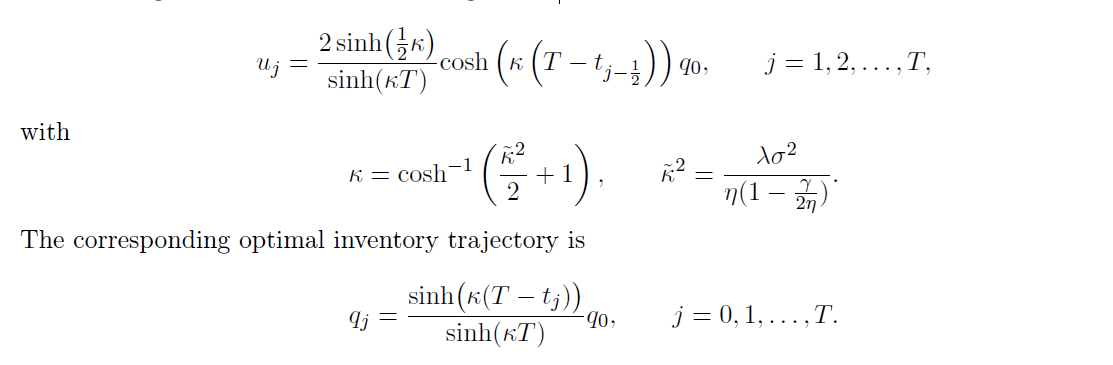
\includegraphics[scale = 0.5]{Stoc3.png}
\end{center}
\end{figure}

Performance and Evaluation : The performance of execution algorithms is evaluated using several criteria such as Profit and Loss (PnL), Implementation Shortfall, and the Sharpe ratio. PnL is the final profit or loss induced by an algorithm over the entire time period. Implementation Shortfall is the difference between the PnL of an algorithm and the PnL received by trading the entire asset instantly. The Sharpe ratio measures return per unit of risk. TWAP and VWAP are popular pre-specified benchmark strategies. The SnL policy involves placing a sell order for all shares at a fixed limit order price, and going to the market with any unexecuted shares remaining at time T.

\subsubsection{RL Approach}
Here we discuss the existing literature on reinforcement learning (RL) methods for optimal execution in trading. Various types of RL algorithms have been employed, including value-based (Q-learning algorithms and double DQN) and policy-based (deep policy gradient methods, A2C, PPO, and DDPG) algorithms. The benchmark strategies studied in these papers include the Almgren–Chriss solution, the TWAP strategy, the VWAP strategy, and the SnL policy. The state variables and control variables used in the RL models are often the market attributes, inventory process, past returns, and amount of asset or relative price level at each time point. The reward functions used include cash inflow or outflow, implementation shortfall, profit, Sharpe ratio, and return.


\subsection{Market Making}
A market maker is a trader or institution that provides liquidity to the market by placing buy and sell limit orders in the LOB for a financial instrument, earning the bid-ask spread. The objective is to profit from the spread without accumulating large positions. Three major sources of risk include inventory risk, execution risk, and adverse selection risk. The market maker seeks to avoid accumulating an undesirably large net inventory, ensuring limit orders get filled over a desired horizon, and preventing directional price movements from causing huge losses.

\subsubsection{Stochastic Control Approach}
An optimal market making strategy that maximizes the market maker’s expected utility can be obtained by solving the Hamilton–Jacobi–Bellman equation

Finally, the market maker optimizes a constant absolute risk aversion (CARA) utility function:
\begin{figure}[H]
\begin{center}
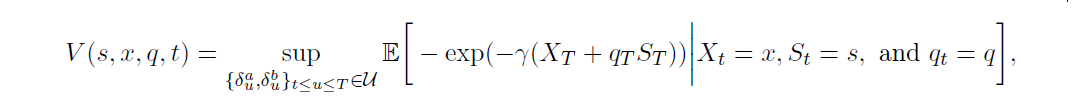
\includegraphics[scale = 0.5]{Stoc1.png}
\end{center}
\end{figure}


By applying the dynamic programming principle, the value function V solves the following Hamilton–Jacobi–Bellman equation:
\begin{figure}[H]
\begin{center}
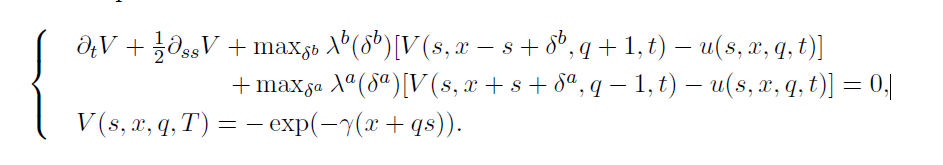
\includegraphics[scale = 0.5]{Stoc2.png}
\end{center}
\end{figure}

This requirement of full analytical specification means these papers are quite removed from realistic market making, as financial markets do not conform to any simple parametric model specification with fixed parameters.


\subsubsection{RL Approach}
RL algorithms such as Q-learning, SARSA, and deep policy gradient have been used, and the state variables include bid and ask prices, current holdings of assets, order-flow imbalance, volatility, and some sophisticated market indices. The control variables are typically set to be the spread to post a pair of limit buy and limit sell orders. The reward function includes parameters such as PnL with inventory cost or Implementation Shortfall with inventory cost. There are different papers that have contributed to improving the RL approach in market making. One such paper explores three RL algorithms, a Monte Carlo method, a SARSA method, and an actor-critic method. Another paper parametrizes a group of "spread-based" market making strategies and uses an online algorithm to pick a minimum quoted spread. Another paper uses Book Exhaustion Rate (BER) to avoid large losses due to adverse selection and achieve stable performance. Finally, some recent papers have focused on improving the robustness of market makers' strategies with respect to adversarial and volatile market conditions.

\subsection{Robo Advising}
Robo-advisors are online financial advisers that use mathematical rules or algorithms to provide investment management with minimal human intervention. They emerged as an alternative to traditional human advisers after the 2008 financial crisis. The robo-advisor learns the client's risk preference while interacting with them and adjusts its investment decisions accordingly. However, there are challenges in determining the frequency of interaction with the client, balancing client preferences with better investment performance, and accurately acquiring information from the client while accounting for their behavioral biases. As of 2020, the value of assets under robo-management is highest in the United States and exceeded 650 billion.

\subsubsection{Stochastic Control Approach}
A stochastic control framework was proposed, consisting of a regime switching model of market returns, a mechanism of interaction between the client and the robo-advisor, a dynamic model for the client's risk preferences, and an optimal investment criterion. The robo-advisor interacts repeatedly with the client to learn about changes in their risk profile, and adopts a multi-period mean-variance investment criterion based on the estimate of the client's risk aversion level. The resulting stock market allocation consists of two components: a standard single period Markowitz strategy and an intertemporal hedging demand. The framework is general enough that some components can be replaced by an RL algorithm, and the dependence on model specification can potentially be relaxed.

\subsubsection{RL Approach}
The use of reinforcement learning (RL) in robo-advising is a relatively new area of research. One of the first proposed RL algorithms for robo-advising, which used an exploration-exploitation algorithm to learn the investor's risk appetite over time by observing her portfolio choices in different market environments. Another proposed investment robo-advising framework consisted of two agents, an inverse portfolio optimization agent, and a deep RL agent that aggregates the inferred sequence of expected returns to formulate a new multi-period mean-variance portfolio optimization problem. Additionally, an inverse optimization technique to measure time-varying risk preferences directly from market signals and portfolios.


\subsection{Further Developments for Mathematical Finance and Reinforcement Learning}
The integration of stochastic control techniques and domain knowledge from financial applications with RL algorithms is a promising direction for RL in finance. This could lead to better empirical performance and potential new frameworks for RL algorithms. Convergence and sample complexity analysis of these modified algorithms would be a meaningful direction to proceed. Many papers provide initial steps in this direction.

\subsubsection{Risk-aware or Risk-sensitive RL}
Risk is inherent in financial decision-making due to uncertainty about future events. To address this, incorporating risk measures into RL algorithms for financial applications is important. Several studies have proposed risk-sensitive RL algorithms with varying degrees of theoretical guarantees and efficiency, including TD(0), Q-learning, policy gradient, and martingale approaches. Other work focuses on constrained RL problems with different risk criteria or robust optimization frameworks with rank dependent expected utility functions. However, sample complexity and asymptotic convergence have not been studied for some of these proposed algorithms. Financial applications such as statistical arbitrage and portfolio optimization are discussed with numerical examples.

\subsubsection{Offline Learning and Online Exploration}
Real-time updating of algorithm parameters is impractical for many financial decision-making problems, particularly in high-frequency trading. Instead, data is typically collected during trading hours with a pre-specified exploration scheme and the algorithm is updated after the close of trading. This approach is related to offline regression and RL with batch data, but these methodologies are not specifically tailored to financial applications and focus on general methodologies.

\subsubsection{Learning with a Limited Exploration Budget}
Exploration can help agents find new policies to improve future cumulative rewards, but excessive exploration can be costly and time-consuming, especially in financial applications where black-box trading strategies may require justification. Investors typically limit exploration efforts and focus on improving performance within a given budget for exploration, similar to the conservative RL approach. This is related to the problem of information acquisition with a cost, which has been studied in other fields and may be relevant for decision-making in financial markets.

\subsubsection{Learning with Multiple Objectives}
Choosing a portfolio in finance involves balancing conflicting objectives of maximizing expected returns while minimizing risk. This is represented by a graph with an efficient frontier and indifference curves showing preferences for risk-expected return combinations. Decision makers often combine criteria into a single objective function, but this may not always be optimal. Market makers on the OTC market view criteria such as turn around time, balance sheet constraints, inventory cost, profit, and loss as separate objectives.

\subsubsection{Learning to Allocate Across Lit Pools and Dark Pools}
There is a lack of existing work on applying multi-period and model-free RL methods to learn how to route orders across both dark pools and lit pools in finance. While there are online optimization and Bayesian methods for allocation across these pools, they do not use RL. Combining both lit and dark pools could present an interesting direction to explore as they have different information structures and matching mechanisms.

\subsubsection{Robo-advising in a Model-free Setting}
There are approaches for learning within a pre-specified set of investment portfolios using Markowitz mean-variance optimization. However, a model-free RL approach where the robo-advisor can learn and improve decisions beyond pre-specified strategies or frameworks would be interesting to explore.

\subsubsection{Sample Efficiency in Learning Trading Strategies}
Recent studies have focused on sample complexity in modern reinforcement learning algorithms for financial applications. However, most algorithms still require a large amount of training data, which may exceed the available historical data. Financial time series are non-stationary, making historical data from further back less relevant for current market conditions. This highlights the need for more sample-efficient RL algorithms or realistic market simulators to generate unlimited market scenarios.

\subsubsection{Transfer Learning and Cold Start for Learning New Assets}
Financial institutions and individuals may change their baskets of assets to trade over time, leading to the need for transferring trading strategies from one asset to another or initializing algorithms for newly issued assets with limited data. Transfer learning techniques have not yet been explored in financial applications for transferring experience from one similar asset to another. The cold-start problem arises when there is limited data available for a newly issued asset, and the challenge is to initialize an RL algorithm and learn a decent trading strategy using the limited available data and experience with other longstanding assets.





\end{document}


